\documentclass[aspectratio=169, handout]{beamer}

%\usepackage[table]{xcolor}
\mode<presentation> {
\setbeamercovered{transparent}
  \usetheme{Boadilla}

\renewcommand{\familydefault}{cmss}
\usepackage{bm}
\usepackage{listings}
\useinnertheme{rectangles}
}
\usepackage{amsmath}
\usepackage{bbold}
\usepackage{tcolorbox}
\setbeamercolor{normal text}{fg=black}
\setbeamercolor{structure}{fg= blue}
\definecolor{trial}{cmyk}{1,0,0, 0}
\definecolor{trial2}{cmyk}{0.00,0,1, 0}
\definecolor{darkgreen}{rgb}{0,.4, 0.1}
\usepackage{array}
\beamertemplatesolidbackgroundcolor{white}  \setbeamercolor{alerted
text}{fg=red}
\setbeamertemplate{caption}[numbered]\newcounter{mylastframe}

\font\domino=domino
\def\die#1{{\domino#1}}
\usepackage{tikz}
\usetikzlibrary{arrows}
\usepackage{colortbl}

\renewcommand{\familydefault}{cmss}

\usepackage{tikz}
\usepackage{lipsum}
\usepackage{booktabs}

\lstset{%
  language=R,
  basicstyle=\ttfamily\small,
  keywordstyle=\color{blue},
  commentstyle=\color{darkgreen},
  stringstyle=\color{red},
  showstringspaces=false,
  breaklines=true,
  frame=single,
  backgroundcolor=\color{gray!10}
}

 \newenvironment{changemargin}[3]{%
 \begin{list}{}{%
 \setlength{\topsep}{0pt}%
 \setlength{\leftmargin}{#1}%
 \setlength{\rightmargin}{#2}%
 \setlength{\topmargin}{#3}%
 \setlength{\listparindent}{\parindent}%
 \setlength{\itemindent}{\parindent}%
 \setlength{\parsep}{\parskip}%
 }%
\item[]}{\end{list}}
\usetikzlibrary{arrows}
\usetikzlibrary{arrows.meta}
\usepackage{pgfplots}
\pgfplotsset{compat=1.17}
\usecolortheme{lily}

\newtheorem{com}{Comment}
\newtheorem{lem} {Lemma}
\newtheorem{prop}{Proposition}
\newtheorem{condition}{Condition}
\newtheorem{thm}{Theorem}
\newtheorem{defn}{Definition}
\newtheorem{cor}{Corollary}
\newtheorem{obs}{Observation}
 \numberwithin{equation}{section}

\makeatletter
\def\beamerorig@set@color{%
  \pdfliteral{\current@color}%
  \aftergroup\reset@color
}
\def\beamerorig@reset@color{\pdfliteral{\current@color}}
\makeatother
\setbeamertemplate{navigation symbols}{}

\useoutertheme{miniframes}
\title[PLSC 30700]{Linear Models Lecture 12: Hypothesis Testing}

\author{Robert Gulotty}
\institute[Chicago]{University of Chicago}
\vspace{0.3in}


\begin{document}

\begin{frame}
\maketitle
\end{frame}

%%%%%%%%%%%%%%%%%%%%%%%%%%%%%%%%%%%%%%%%%%%%%%%%%%%%%%%%%%%%
\begin{frame}{Where We Are}

\textbf{Last lecture:} We derived the Wald statistic
$$W = (\bm{R}\hat{\bm{\beta}} - \bm{r})'\left[\bm{R}\hat{\bm{V}}\bm{R}'\right]^{-1}(\bm{R}\hat{\bm{\beta}} - \bm{r}) \;\xrightarrow{d}\; \chi^2_q$$
and showed how to construct robust tests and confidence intervals.

\pause
\bigskip

\textbf{Today:} We go deeper into the \emph{practice} of hypothesis testing.

\begin{itemize}
\item The F test: a criterion-based alternative
\item Score (LM) tests: testing from the restricted model
\item The trinity of classical tests
\item Test inversion for confidence regions
\item Multiple testing and Bonferroni corrections
\item Power: what determines whether you can detect an effect?
\item Hansen's practical advice for applied work
\end{itemize}
\end{frame}

%%%%%%%%%%%%%%%%%%%%%%%%%%%%%%%%%%%%%%%%%%%%%%%%%%%%%%%%%%%%
\section{Constrained LS}
\setcounter{subsection}{1}
%%%%%%%%%%%%%%%%%%%%%%%%%%%%%%%%%%%%%%%%%%%%%%%%%%%%%%%%%%%%

%%%%%%%%%%%%%%%%%%%%%%%%%%%%%%%%%%%%%%%%%%%%%%%%%%%%%%%%%%%%
\begin{frame}{Constrained Least Squares: Setup}

Many tests today compare an \textbf{unrestricted} model to a \textbf{restricted} one.  We need to know how to estimate under restrictions.

\pause
\bigskip

\textbf{Problem:} Minimize the sum of squared errors subject to $q$ linear constraints:
$$\tilde{\bm{\beta}}_{\text{CLS}} = \arg\min_{\bm{\beta}} \sum_{i=1}^n (Y_i - \bm{X}_i'\bm{\beta})^2 \quad \text{subject to} \quad \bm{R}'\bm{\beta} = \bm{r}$$

where $\bm{R}$ is $k \times q$ and $\bm{r}$ is $q \times 1$.

\pause
\bigskip

\textbf{Examples:}
\begin{itemize}
\item $\beta_3 = 0$: set $\bm{R}' = (0, 0, 1, 0, \ldots)$, $\bm{r} = 0$ \quad (exclusion restriction)
\item $\beta_2 = \beta_3$: set $\bm{R}' = (0, 1, -1, 0, \ldots)$, $\bm{r} = 0$ \quad (equality restriction)
\item $\beta_2 + \beta_3 = 1$: set $\bm{R}' = (0, 1, 1, 0, \ldots)$, $\bm{r} = 1$ \quad (adding-up constraint)
\end{itemize}
\end{frame}

%%%%%%%%%%%%%%%%%%%%%%%%%%%%%%%%%%%%%%%%%%%%%%%%%%%%%%%%%%%%
\begin{frame}{The CLS Estimator}

Solve via Lagrange multipliers.  The solution is:

$$\boxed{\tilde{\bm{\beta}}_{\text{CLS}} = \hat{\bm{\beta}}_{\text{OLS}} - (\bm{X}'\bm{X})^{-1}\bm{R}\left[\bm{R}'(\bm{X}'\bm{X})^{-1}\bm{R}\right]^{-1}(\bm{R}'\hat{\bm{\beta}}_{\text{OLS}} - \bm{r})}$$

\pause
\smallskip

\textbf{Reading the formula:}
\begin{itemize}
\item Start from unrestricted OLS $\hat{\bm{\beta}}_{\text{OLS}}$, subtract a correction toward the constraint
\item Correction is proportional to $(\bm{R}'\hat{\bm{\beta}}_{\text{OLS}} - \bm{r})$: how far OLS violates $H_0$
\item If OLS already satisfies the restriction, $\tilde{\bm{\beta}}_{\text{CLS}} = \hat{\bm{\beta}}_{\text{OLS}}$
\end{itemize}

\pause
\smallskip

The restricted residuals and variance estimate are:
$$\tilde{e}_i = Y_i - \bm{X}_i'\tilde{\bm{\beta}}_{\text{CLS}}, \qquad \tilde{\sigma}^2 = \frac{1}{n}\sum_{i=1}^n \tilde{e}_i^2$$

Since the restriction constrains the parameter space: $\tilde{\sigma}^2 \geq \hat{\sigma}^2$ always.
\end{frame}

%%%%%%%%%%%%%%%%%%%%%%%%%%%%%%%%%%%%%%%%%%%%%%%%%%%%%%%%%%%%
\begin{frame}[fragile]{CLS in Practice}

\textbf{Simple case:} If $H_0$ sets some coefficients to zero, CLS just means dropping those regressors.

\begin{lstlisting}
# Unrestricted
mod_U <- lm(lwage ~ education + exper + I(exper^2) +
              female + union, data = wages)
# Restricted (H0: beta_female = beta_union = 0)
mod_R <- lm(lwage ~ education + exper + I(exper^2),
              data = wages)
\end{lstlisting}

\pause
\smallskip

\textbf{General case:} For arbitrary linear restrictions (e.g., $\beta_2 = \beta_3$), reparameterize or use the closed-form formula.

\pause
\smallskip

\begin{tcolorbox}[colback=blue!5, colframe=blue!50]
The key outputs from CLS are $\text{SSE}_R = \sum \tilde{e}_i^2$ and $\tilde{\sigma}^2$, which we use to build the F and Score statistics.
\end{tcolorbox}
\end{frame}

%%%%%%%%%%%%%%%%%%%%%%%%%%%%%%%%%%%%%%%%%%%%%%%%%%%%%%%%%%%%
\section{The F Test}
\setcounter{subsection}{1}
%%%%%%%%%%%%%%%%%%%%%%%%%%%%%%%%%%%%%%%%%%%%%%%%%%%%%%%%%%%%

%%%%%%%%%%%%%%%%%%%%%%%%%%%%%%%%%%%%%%%%%%%%%%%%%%%%%%%%%%%%
\begin{frame}{The F Test: Idea}

The F test asks: \textbf{how much does the fit worsen when we impose the null?}

\pause
\bigskip

\begin{itemize}
\item Run the \textbf{unrestricted} regression: get $\text{SSE}_U = \sum(Y_i - \bm{X}_i'\hat{\bm{\beta}}_{\text{OLS}})^2$
\item Run the \textbf{restricted} regression (imposing $H_0$): get $\text{SSE}_R = \sum(Y_i - \bm{X}_i'\tilde{\bm{\beta}}_{\text{CLS}})^2$

\pause
\bigskip
\item Since $H_0$ constrains the parameter space, $\text{SSE}_R \geq \text{SSE}_U$ always.
\item If the fit barely worsens $\Rightarrow$ the restriction is consistent with the data.
\item If the fit worsens a lot $\Rightarrow$ the restriction is costly $\Rightarrow$ evidence against $H_0$.
\end{itemize}
\end{frame}

%%%%%%%%%%%%%%%%%%%%%%%%%%%%%%%%%%%%%%%%%%%%%%%%%%%%%%%%%%%%
\begin{frame}{The F Statistic}

Testing $H_0\colon \bm{R}'\bm{\beta} = \bm{r}$ with $q$ restrictions:

$$\boxed{F = \frac{(\text{SSE}_R - \text{SSE}_U)/q}{\text{SSE}_U/(n-k)} = \frac{(\tilde{\sigma}^2 - \hat{\sigma}^2)/q}{\hat{\sigma}^2/(n-k)}}$$

\pause
\smallskip

\begin{itemize}
\item \textbf{Numerator}: average increase in residual variance per restriction
\item \textbf{Denominator}: unrestricted estimate of error variance ($s^2$)
\item Reject $H_0$ when $F$ is large
\end{itemize}

\pause
\smallskip

\begin{tcolorbox}[colback=blue!5, colframe=blue!50]
\textbf{Key relationship:} For linear hypotheses, $F = W^0 / q$ where $W^0$ is the homoskedastic Wald statistic.  Under homoskedasticity and normality, $F \sim F_{q,\,n-k}$ exactly. Asymptotically, $F \xrightarrow{d} \chi^2_q/q$.
\end{tcolorbox}
\end{frame}

%%%%%%%%%%%%%%%%%%%%%%%%%%%%%%%%%%%%%%%%%%%%%%%%%%%%%%%%%%%%
\begin{frame}{F Test: When and Why}

\textbf{Advantages:}
\begin{itemize}
\item Directly computable from standard output (just need SSE from two regressions)
\item Exact distribution under normality + homoskedasticity
\item Slightly more conservative than $\chi^2$ critical values (good in small samples)
\end{itemize}

\pause
\smallskip

\textbf{Limitations:}
\begin{itemize}
\item Requires homoskedasticity for the $F_{q,n-k}$ distribution to be valid
\item Under heteroskedasticity, use the robust Wald test from Lecture~11 instead
\end{itemize}

\pause
\smallskip

\begin{tcolorbox}[colback=red!5, colframe=red!50]
\textbf{Hansen's warning:} Many packages automatically report an ``F-statistic'' testing that all slopes are zero.  With modern sample sizes this is nearly always significant. \textbf{There is no reason to report this F statistic.}
\end{tcolorbox}
\end{frame}

%%%%%%%%%%%%%%%%%%%%%%%%%%%%%%%%%%%%%%%%%%%%%%%%%%%%%%%%%%%%
\begin{frame}[fragile]{F Test in R}
\begin{lstlisting}
mod_U <- lm(lwage ~ education + exper + I(exper^2) +
              female + union, data = wages)
mod_R <- lm(lwage ~ education + exper + I(exper^2),
              data = wages)

# Manual F test
SSE_U <- sum(resid(mod_U)^2)
SSE_R <- sum(resid(mod_R)^2)
q <- 2; n <- nobs(mod_U); k <- length(coef(mod_U))
F_stat <- ((SSE_R - SSE_U)/q) / (SSE_U/(n - k))
p_val  <- 1 - pf(F_stat, q, n - k)

# Or simply:
anova(mod_R, mod_U)
\end{lstlisting}
\end{frame}

%%%%%%%%%%%%%%%%%%%%%%%%%%%%%%%%%%%%%%%%%%%%%%%%%%%%%%%%%%%%
\begin{frame}{Example: Joint Significance}

Wage regression with ``Male Union Member'' and ``Female Union Member'' indicators.

\bigskip
\textbf{Test:} $H_0$: Union membership has no effect on wages (both coefficients = 0).

\pause
\bigskip

\begin{itemize}
\item $W = 23$ (Wald), so $F = 23/2 = 11.5$, $p < 0.001$. \textbf{Reject.}
\end{itemize}

\pause
\bigskip

\begin{tcolorbox}[colback=blue!5, colframe=blue!50]
\textbf{Interpretation:} Rejecting the joint null means \emph{at least one} coefficient is nonzero. It does not mean both are.  Always examine both the joint test and individual t-statistics for a complete picture.
\end{tcolorbox}
\end{frame}

%%%%%%%%%%%%%%%%%%%%%%%%%%%%%%%%%%%%%%%%%%%%%%%%%%%%%%%%%%%%
\section{Score Tests}
\setcounter{subsection}{1}
%%%%%%%%%%%%%%%%%%%%%%%%%%%%%%%%%%%%%%%%%%%%%%%%%%%%%%%%%%%%

%%%%%%%%%%%%%%%%%%%%%%%%%%%%%%%%%%%%%%%%%%%%%%%%%%%%%%%%%%%%
\begin{frame}{Score Tests: The Idea}

The Wald test starts from the \textbf{unrestricted} estimate and asks: is $\hat{\bm{\theta}}$ far from $\bm{\theta}_0$?

\pause
\bigskip

The \textbf{Score test} (also called \textbf{Lagrange Multiplier test}) starts from the \textbf{restricted} estimate and asks: does the objective function want to move away from the restriction?

\pause
\bigskip

\begin{itemize}
\item Compute the restricted estimator $\tilde{\bm{\beta}}$ (constrained least squares)
\item Evaluate the \emph{gradient} (score) of the objective function at $\tilde{\bm{\beta}}$
\item If $H_0$ is true, the score should be near zero (we're near the optimum)
\item If $H_0$ is false, the score should be large (the restriction is pulling us away)
\end{itemize}
\end{frame}

%%%%%%%%%%%%%%%%%%%%%%%%%%%%%%%%%%%%%%%%%%%%%%%%%%%%%%%%%%%%
\begin{frame}{Score Statistic for Linear Restrictions}

For $H_0\colon \bm{R}'\bm{\beta} = \bm{c}$ in the normal regression model:

$$S = \frac{(\bm{R}'\hat{\bm{\beta}} - \bm{c})'[\bm{R}'(\bm{X}'\bm{X})^{-1}\bm{R}]^{-1}(\bm{R}'\hat{\bm{\beta}} - \bm{c})}{\tilde{\sigma}^2}$$

\pause

\begin{itemize}
\item Identical to $W^0$ except $s^2$ replaced by $\tilde{\sigma}^2$ (restricted variance).
\item Under $H_0$: $S \xrightarrow{d} \chi^2_q$
\end{itemize}

\pause

\begin{tcolorbox}[colback=blue!5, colframe=blue!50]
\textbf{Key result:} $S$ is a monotone transformation of $F$:
$S = n\left(1 - \frac{1}{1 + qF/(n-k)}\right)$,
so the Score test and the F test always give the same accept/reject decision.
\end{tcolorbox}
\end{frame}

%%%%%%%%%%%%%%%%%%%%%%%%%%%%%%%%%%%%%%%%%%%%%%%%%%%%%%%%%%%%
\begin{frame}{When Are Score Tests Useful?}

For linear regression with linear restrictions, the Score test offers nothing new over $F$ or Wald.

\pause
\smallskip

\textbf{But} in more complex settings, Score tests have a major advantage:

\begin{itemize}
\item They only require estimation under $H_0$ (the restricted model)
\item The ``unrestricted'' model may not even be a simple OLS regression
\end{itemize}

\pause
\smallskip

\textbf{Example:} Testing for heteroskedasticity (Breusch--Pagan).  The null is homoskedastic OLS---easy.  The unrestricted model allows $\text{Var}(e_i \mid X_i)$ to vary with $X$, which requires modeling the variance function.  The Score test only needs the OLS residuals.

\pause
\smallskip

\textbf{Same idea applies to:}
\begin{itemize}
\item Testing for serial correlation (Breusch--Godfrey): null is OLS with iid errors
\item Testing for omitted nonlinearities: null is a simple linear specification
\item Any setting where $H_0$ gives you a clean model but $H_1$ is messy
\end{itemize}
\end{frame}

%%%%%%%%%%%%%%%%%%%%%%%%%%%%%%%%%%%%%%%%%%%%%%%%%%%%%%%%%%%%
\section{The Trinity}
\setcounter{subsection}{1}
%%%%%%%%%%%%%%%%%%%%%%%%%%%%%%%%%%%%%%%%%%%%%%%%%%%%%%%%%%%%

%%%%%%%%%%%%%%%%%%%%%%%%%%%%%%%%%%%%%%%%%%%%%%%%%%%%%%%%%%%%
\begin{frame}{Three Ways to Test the Same Hypothesis}

\begin{center}
\renewcommand{\arraystretch}{1.2}
\begin{tabular}{lccc}
\toprule
 & \textbf{Wald} & \textbf{Score (LM)} & \textbf{F / LR-like} \\
\midrule
\textbf{Estimates from} & Unrestricted & Restricted & Both \\
\textbf{Measures} & Distance of $\hat{\bm{\theta}}$ & Gradient at & Change in \\
 & from $\bm{\theta}_0$ & restriction & fit (SSE) \\
\textbf{Null dist.} & $\chi^2_q$ & $\chi^2_q$ & $\chi^2_q/q$ or $F_{q,n-k}$ \\
\textbf{Robust?} & Yes (sandwich) & Score-like & No \\
\bottomrule
\end{tabular}
\end{center}

\pause

\begin{tcolorbox}[colback=blue!5, colframe=blue!50]
For linear restrictions in the normal model, all three are monotone transformations of each other and give identical decisions. They differ for nonlinear restrictions or non-normal models.
\end{tcolorbox}
\end{frame}

%%%%%%%%%%%%%%%%%%%%%%%%%%%%%%%%%%%%%%%%%%%%%%%%%%%%%%%%%%%%
\begin{frame}{Visualizing the Trinity}

\begin{center}
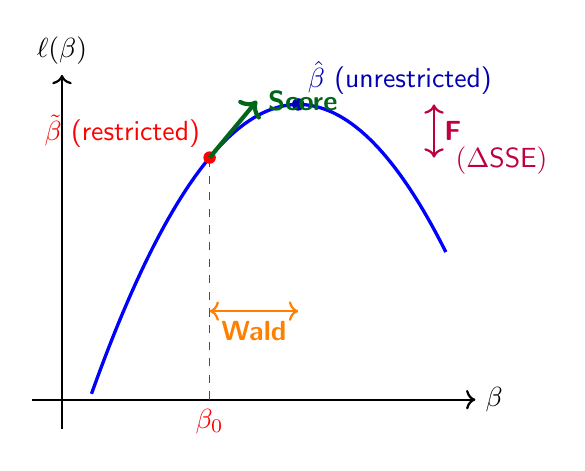
\begin{tikzpicture}[scale=0.75]
  % Axes
  \draw[->, thick] (-0.5,0) -- (7,0) node[right] {$\beta$};
  \draw[->, thick] (0,-0.5) -- (0,5.5) node[above] {$\ell(\beta)$};
  % Log-likelihood curve
  \draw[blue, very thick, domain=0.5:6.5, samples=80]
    plot (\x, {5 - 0.4*(\x - 4)^2});
  % Points
  \fill[red] (2.5, {5 - 0.4*(2.5-4)^2}) circle (3pt)
    node[above left] {$\tilde{\beta}$ (restricted)};
  \fill[blue!70!black] (4, 5) circle (3pt)
    node[above right] {$\hat{\beta}$ (unrestricted)};
  % Null value
  \draw[dashed, red] (2.5, 0) -- (2.5, {5 - 0.4*(2.5-4)^2});
  \node[below, red] at (2.5, 0) {$\beta_0$};
  % Wald arrow
  \draw[<->, thick, orange] (2.5, 1.5) -- (4, 1.5)
    node[midway, below] {\textbf{Wald}};
  % Score arrow (tangent)
  \draw[->, thick, darkgreen, line width=1.5pt] (2.5, {5 - 0.4*(2.5-4)^2})
    -- ++(0.8, {0.8*0.8*(4-2.5)})
    node[right] {\textbf{Score}};
  % F / criterion arrow
  \draw[<->, thick, purple] (6.3, {5 - 0.4*(2.5-4)^2}) -- (6.3, 5)
    node[midway, right] {\textbf{F}};
  \node[purple, right] at (6.5, {(5 + 5 - 0.4*(2.5-4)^2)/2 - 0.5}) {$(\Delta\text{SSE})$};
\end{tikzpicture}
\end{center}

\vspace{-0.3cm}
\begin{itemize}
\item \textbf{\color{orange}Wald}: horizontal distance between $\hat{\beta}$ and $\beta_0$ \quad \textbf{\color{darkgreen}Score}: slope at restricted estimate \quad \textbf{\color{purple}F}: vertical distance ($\Delta$SSE)
\end{itemize}
\end{frame}

%%%%%%%%%%%%%%%%%%%%%%%%%%%%%%%%%%%%%%%%%%%%%%%%%%%%%%%%%%%%
\section{Test Inversion}
\setcounter{subsection}{1}
%%%%%%%%%%%%%%%%%%%%%%%%%%%%%%%%%%%%%%%%%%%%%%%%%%%%%%%%%%%%

%%%%%%%%%%%%%%%%%%%%%%%%%%%%%%%%%%%%%%%%%%%%%%%%%%%%%%%%%%%%
\begin{frame}{Confidence Intervals \emph{Are} Inverted Tests}

Recall the standard 95\% CI:
$$\hat{C} = \left[\hat{\theta} - 1.96\cdot s(\hat{\theta}),\;\; \hat{\theta} + 1.96\cdot s(\hat{\theta})\right]$$

\pause

This is exactly the set of values $\theta$ that are \emph{not rejected} by a two-sided $t$-test:
$$\hat{C} = \left\{\theta \;:\; |T(\theta)| \leq 1.96\right\}$$

\pause
\bigskip

\begin{tcolorbox}[colback=blue!5, colframe=blue!50]
\textbf{General principle:} Inverting a test with good Type~I error control produces a confidence set with good coverage.
$$P[\theta \in \hat{C}] = P[\text{Accept}\mid \theta] = 1 - P[\text{Type I error}]$$
\end{tcolorbox}
\end{frame}

%%%%%%%%%%%%%%%%%%%%%%%%%%%%%%%%%%%%%%%%%%%%%%%%%%%%%%%%%%%%
\begin{frame}{Why Test Inversion Matters: Nonlinear Parameters}

Consider $\theta = \beta_1 / \beta_2$ (e.g., peak experience in a wage equation).

\pause
\bigskip

\textbf{Approach 1:} Delta method CI
$$\hat{\theta} \pm 1.96 \cdot s(\hat{\theta})$$
From Lecture~11, this can be inaccurate for ratios (Fieller's problem).

\pause
\bigskip

\textbf{Approach 2:} Rewrite as a \emph{linear} restriction $\beta_1 - \theta\beta_2 = 0$ and invert:
$$\hat{C} = \left\{\theta \;:\; \frac{(\hat{\beta}_1 - \theta\hat{\beta}_2)^2}{\bm{R}'(\theta)\hat{\bm{V}}\bm{R}(\theta)} \leq 1.96^2\right\}$$
where $\bm{R}(\theta) = (1, -\theta)'$.  This requires a grid search over $\theta$.

\pause
\bigskip

\textbf{Hansen's example:}  Peak experience $= -50\beta_1/\beta_2$.\\
Delta method CI: $[29.8,\; 29.9]$. \quad Inverted linear test CI: $[29.1,\; 30.6]$.\\
The delta method interval is \textbf{far too narrow}.
\end{frame}

%%%%%%%%%%%%%%%%%%%%%%%%%%%%%%%%%%%%%%%%%%%%%%%%%%%%%%%%%%%%
\begin{frame}[fragile]{Test Inversion in R}
\begin{lstlisting}
# Wage equation: log(wage) ~ exper + exper^2/100 + ...
mod <- lm(lwage ~ exper + I(exper^2/100) + education,
           data = wages)
b <- coef(mod); V <- vcovHC(mod)

# Grid search: invert the t-test for theta = -50*b1/b2
theta_grid <- seq(20, 40, by = 0.01)
in_CI <- sapply(theta_grid, function(th) {
  R <- c(0, 1, -th/50, 0)  # gradient of b[2] - th*b[3]/50
  num <- (b[2] - th * b[3] / 50)^2
  den <- t(R) %*% V %*% R
  num / den <= qchisq(0.95, 1)
})
CI <- range(theta_grid[in_CI])
\end{lstlisting}
\end{frame}

%%%%%%%%%%%%%%%%%%%%%%%%%%%%%%%%%%%%%%%%%%%%%%%%%%%%%%%%%%%%
\begin{frame}{Confidence Regions for Multiple Parameters}

For $q > 1$ parameters, invert the Wald test:
$\hat{C} = \left\{\bm{\theta} : W(\bm{\theta}) \leq \chi^2_{q,\,1-\alpha}\right\}$
--- an \textbf{ellipsoid} in $\mathbb{R}^q$ centered at $\hat{\bm{\theta}}$, shaped by $\hat{\bm{V}}_\theta^{-1}$.

\pause

\begin{center}
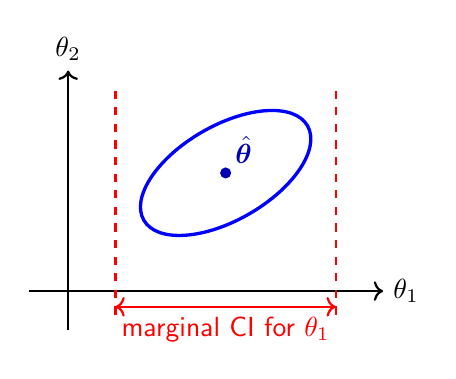
\begin{tikzpicture}[scale=1.0]
  \draw[->, thick] (-0.5,0) -- (4,0) node[right] {$\theta_1$};
  \draw[->, thick] (0,-0.5) -- (0,2.8) node[above] {$\theta_2$};
  % Ellipse
  \draw[blue, very thick, rotate around={30:(2,1.5)}] (2,1.5) ellipse (1.2 and 0.6);
  \fill[blue!70!black] (2,1.5) circle (2pt) node[above right] {$\hat{\bm{\theta}}$};
  % Marginal intervals
  \draw[red, dashed, thick] (0.6, -0.3) -- (0.6, 2.6);
  \draw[red, dashed, thick] (3.4, -0.3) -- (3.4, 2.6);
  \draw[<->, red, thick] (0.6, -0.2) -- (3.4, -0.2) node[midway, below] {marginal CI for $\theta_1$};
\end{tikzpicture}
\end{center}

\vspace{-0.3cm}
Marginal CIs (projections) are always wider than the ellipsoid in each dimension.
\end{frame}

%%%%%%%%%%%%%%%%%%%%%%%%%%%%%%%%%%%%%%%%%%%%%%%%%%%%%%%%%%%%
\section{Bonferroni}
\setcounter{subsection}{1}
%%%%%%%%%%%%%%%%%%%%%%%%%%%%%%%%%%%%%%%%%%%%%%%%%%%%%%%%%%%%

%%%%%%%%%%%%%%%%%%%%%%%%%%%%%%%%%%%%%%%%%%%%%%%%%%%%%%%%%%%%
\begin{frame}{The Multiple Testing Problem}

Suppose you test $k$ hypotheses, each at level $\alpha = 0.05$.  Under the \textbf{global null} (all $k$ true), what is $P[\text{at least one false rejection}]$?

\pause
\smallskip

By \textbf{Boole's inequality}:
$$P\!\left[\min_{j \leq k} p_j < \alpha\right] \;\leq\; \sum_{j=1}^k P[p_j < \alpha] \;\to\; k\alpha$$

\pause

\begin{center}
\renewcommand{\arraystretch}{1.2}
\begin{tabular}{ccc}
\toprule
$k$ (tests) & $\alpha$ per test & Familywise error $\leq$ \\
\midrule
5 & 0.05 & 0.25 \\
10 & 0.05 & 0.50 \\
20 & 0.05 & 1.00 \\
\bottomrule
\end{tabular}
\end{center}

With 20 tests, you are \emph{virtually certain} to get a false rejection!
\end{frame}

%%%%%%%%%%%%%%%%%%%%%%%%%%%%%%%%%%%%%%%%%%%%%%%%%%%%%%%%%%%%
\begin{frame}{The Bonferroni Correction}

\textbf{Goal:} Control the \emph{familywise error rate} (FWER) at $\alpha$.

\pause
\smallskip

\textbf{Rule:} Reject the $j$th hypothesis only if $p_j < \alpha / k$. \quad Equivalently: $p_{\text{Bonf}} = k \cdot \min_{j \leq k}\; p_j$.

\pause
\smallskip

\textbf{Proof:}
$$P\!\left[\min_{j \leq k} p_j < \frac{\alpha}{k}\right] \;\leq\; \sum_{j=1}^k P\!\left[p_j < \frac{\alpha}{k}\right] \;\to\; k \cdot \frac{\alpha}{k} = \alpha$$

\pause
\smallskip

\begin{tcolorbox}[colback=blue!5, colframe=blue!50]
\textbf{Simple and conservative.}  Controls FWER for \emph{any} dependence structure among the tests.  The cost: reduced power when $k$ is large.
\end{tcolorbox}
\end{frame}

%%%%%%%%%%%%%%%%%%%%%%%%%%%%%%%%%%%%%%%%%%%%%%%%%%%%%%%%%%%%
\begin{frame}{Bonferroni: Worked Example}

Two coefficients tested at $\alpha = 0.05$:

\smallskip
\begin{center}
\renewcommand{\arraystretch}{1.2}
\begin{tabular}{lcc}
\toprule
& Individual $p$ & Bonferroni $p$ ($= 2 \times p$) \\
\midrule
Union membership & 0.04 & 0.08 \\
Married status & 0.15 & 0.30 \\
\bottomrule
\end{tabular}
\end{center}

\pause
\smallskip

\begin{itemize}
\item \textbf{Without correction:} Union membership ``significant'' at 5\%.
\item \textbf{With Bonferroni:} Neither significant at FWER $= 0.05$ (need $p < 0.025$).
\end{itemize}

\pause
\smallskip

\textbf{When to worry:} exploring many specifications/subgroups, examining many coefficients, or reporting the ``most significant'' result.
\end{frame}

%%%%%%%%%%%%%%%%%%%%%%%%%%%%%%%%%%%%%%%%%%%%%%%%%%%%%%%%%%%%
\begin{frame}[fragile]{Bonferroni in R}
\begin{lstlisting}
# Get p-values from a regression
mod <- lm(lwage ~ education + exper + I(exper^2) +
            female + union + married, data = wages)
pvals <- summary(mod)$coefficients[-1, 4]  # drop intercept

# Bonferroni correction
p_bonf <- p.adjust(pvals, method = "bonferroni")
cbind(raw = round(pvals, 4), bonferroni = round(p_bonf, 4))

# Other options: Holm (less conservative, still controls FWER)
p_holm <- p.adjust(pvals, method = "holm")
\end{lstlisting}

\pause
\smallskip
\textbf{Holm's method} is uniformly more powerful than Bonferroni while still controlling FWER.  Use it when available.
\end{frame}

%%%%%%%%%%%%%%%%%%%%%%%%%%%%%%%%%%%%%%%%%%%%%%%%%%%%%%%%%%%%
\section{Power}
\setcounter{subsection}{1}
%%%%%%%%%%%%%%%%%%%%%%%%%%%%%%%%%%%%%%%%%%%%%%%%%%%%%%%%%%%%

%%%%%%%%%%%%%%%%%%%%%%%%%%%%%%%%%%%%%%%%%%%%%%%%%%%%%%%%%%%%
\begin{frame}{Type I and Type II Errors}

\begin{center}
\renewcommand{\arraystretch}{1.3}
\begin{tabular}{lcc}
\toprule
& \textbf{$H_0$ true} & \textbf{$H_0$ false} \\
\midrule
\textbf{Reject $H_0$} & Type I error ($\alpha$) & \textcolor{darkgreen}{Correct (Power $= 1 - \beta$)} \\
\textbf{Accept $H_0$} & \textcolor{darkgreen}{Correct ($1-\alpha$)} & Type II error ($\beta$) \\
\bottomrule
\end{tabular}
\end{center}

\pause

\begin{itemize}
\item \textbf{Size} ($\alpha$): probability of falsely rejecting a true null
\item \textbf{Power} ($\pi$): probability of correctly rejecting a false null: $\pi(\theta) = P[\text{Reject } H_0 \mid \theta \neq \theta_0]$
\item Power depends on the \emph{true value} of $\theta$, on $n$, and on $\alpha$.
\end{itemize}

\pause

\begin{tcolorbox}[colback=red!5, colframe=red!50]
\textbf{Key trade-off:} Making $\alpha$ smaller reduces Type I errors but also reduces power.  A test with $\alpha = 0$ never rejects and has zero power.
\end{tcolorbox}
\end{frame}

%%%%%%%%%%%%%%%%%%%%%%%%%%%%%%%%%%%%%%%%%%%%%%%%%%%%%%%%%%%%
\begin{frame}{Power of the $t$-Test}

For $H_0\colon \theta = \theta_0$ vs.\ $H_1\colon \theta > \theta_0$:

$$T = \frac{\hat{\theta} - \theta_0}{s(\hat{\theta})} \;\approx\; Z + \delta, \quad Z \sim N(0,1)$$

where $\delta = (\theta - \theta_0)/s(\hat{\theta})$ is the \textbf{signal-to-noise ratio}.

\pause
\smallskip

Power of a one-sided test at level $\alpha$: \quad $\pi(\delta) = \Phi(\delta - z_\alpha)$

\pause
\smallskip

\textbf{Power increases when:}
\begin{itemize}
\item The true effect $|\theta - \theta_0|$ is larger
\item The standard error $s(\hat{\theta})$ is smaller (more precise estimation)
\item The significance level $\alpha$ is larger (less stringent threshold)
\item The sample size $n$ is larger (since $s(\hat{\theta}) \propto 1/\sqrt{n}$)
\end{itemize}
\end{frame}

%%%%%%%%%%%%%%%%%%%%%%%%%%%%%%%%%%%%%%%%%%%%%%%%%%%%%%%%%%%%
\begin{frame}{Visualizing Power}

\begin{center}
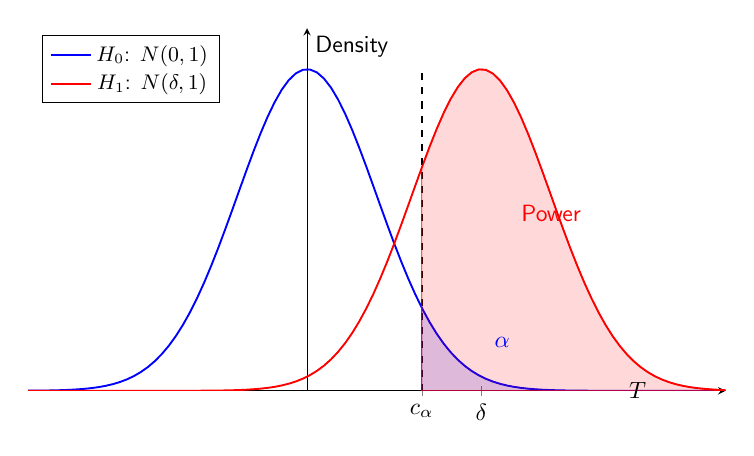
\begin{tikzpicture}[scale=0.85]
  \begin{axis}[
    width=12cm, height=7cm,
    domain=-4:6,
    samples=100,
    xlabel={$T$},
    ylabel={Density},
    ymin=0, ymax=0.45,
    legend style={at={(0.02,0.98)}, anchor=north west, font=\small},
    xtick={0, 1.645, 2.5},
    xticklabels={$0$, $c_\alpha$, $\delta$},
    ytick=\empty,
    axis lines=middle,
    every axis x label/.style={at={(current axis.right of origin)}, anchor=west},
  ]
  % Null distribution
  \addplot[blue, thick] {exp(-x^2/2)/sqrt(2*pi)};
  \addlegendentry{$H_0$: $N(0,1)$}
  % Alternative distribution
  \addplot[red, thick] {exp(-(x-2.5)^2/2)/sqrt(2*pi)};
  \addlegendentry{$H_1$: $N(\delta,1)$}
  % Critical value line
  \draw[dashed, thick, black] (axis cs:1.645,0) -- (axis cs:1.645,0.4);
  % Shaded rejection region under null (Type I)
  \addplot[blue, fill=blue, fill opacity=0.15, domain=1.645:6]
    {exp(-x^2/2)/sqrt(2*pi)} \closedcycle;
  % Shaded power region under alternative
  \addplot[red, fill=red, fill opacity=0.15, domain=1.645:6]
    {exp(-(x-2.5)^2/2)/sqrt(2*pi)} \closedcycle;
  % Labels
  \node[blue] at (axis cs:2.8, 0.06) {$\alpha$};
  \node[red] at (axis cs:3.5, 0.22) {Power};
  \end{axis}
\end{tikzpicture}
\end{center}
\end{frame}

%%%%%%%%%%%%%%%%%%%%%%%%%%%%%%%%%%%%%%%%%%%%%%%%%%%%%%%%%%%%
\begin{frame}{Power in OLS: What You Can Control}

In OLS, $s(\hat{\theta}) \approx \sigma_e / (\text{sd}(X) \cdot \sqrt{n})$ for a single regressor. So:

$$\delta \approx \frac{(\theta - \theta_0) \cdot \text{sd}(X) \cdot \sqrt{n}}{\sigma_e}$$

\pause
\smallskip

\textbf{Levers for increasing power:}
\begin{enumerate}
\item \textbf{Increase $n$}: power grows with $\sqrt{n}$
\item \textbf{Reduce $\sigma_e$}: add controls that explain $Y$ (reduce residual variance)
\item \textbf{Increase $\text{sd}(X)$}: more variation in the regressor of interest
\item \textbf{Increase $\alpha$}: use 5\% instead of 1\% (but more Type I errors)
\end{enumerate}

\pause
\smallskip

\begin{tcolorbox}[colback=blue!5, colframe=blue!50]
\textbf{Controls help power!} Relevant covariates reduce $\sigma_e$ without reducing $\text{sd}(X)$---a free power boost.  But irrelevant covariates cost degrees of freedom.
\end{tcolorbox}
\end{frame}

%%%%%%%%%%%%%%%%%%%%%%%%%%%%%%%%%%%%%%%%%%%%%%%%%%%%%%%%%%%%
\begin{frame}{Power and Test Dimension}

For joint tests ($q > 1$), the Wald statistic under local alternatives:
$W \xrightarrow{d} \chi^2_q(\lambda)$, where $\lambda = \bm{h}'\bm{V}_\theta^{-1}\bm{h}$ is the \textbf{non-centrality parameter}.

\pause
\smallskip

\textbf{Critical fact:} For a fixed $\lambda$, power \emph{decreases} as $q$ increases.

\pause

\begin{center}
\renewcommand{\arraystretch}{1.2}
\begin{tabular}{ccc}
\toprule
$q$ (restrictions) & $\lambda$ for 50\% power & Sample size increase \\
\midrule
1 & 3.85 & baseline \\
2 & 4.96 & $+28\%$ \\
3 & 5.77 & $+50\%$ \\
\bottomrule
\end{tabular}
\end{center}

\pause
\smallskip

\textbf{Takeaway:} Testing more restrictions simultaneously dilutes power.  A single-coefficient $t$-test is more powerful than a joint $F$-test that includes other restrictions.
\end{frame}

%%%%%%%%%%%%%%%%%%%%%%%%%%%%%%%%%%%%%%%%%%%%%%%%%%%%%%%%%%%%
\begin{frame}{The 50\% Power Benchmark}

How far must the true parameter be from $\theta_0$ for 50\% power?

\pause
\smallskip

\textbf{One-sided test:}
\begin{itemize}
\item At $\alpha = 0.05$: need $\delta \geq 1.65$ standard errors
\item At $\alpha = 0.01$: need $\delta \geq 2.33$ standard errors
\end{itemize}

\pause
\smallskip

\textbf{Implication for sample size:}  $(2.33/1.65)^2 \approx 2$.

\begin{tcolorbox}[colback=blue!5, colframe=blue!50]
A test at $\alpha = 0.01$ requires roughly \textbf{twice the sample size} as $\alpha = 0.05$ to achieve the same power.
\end{tcolorbox}

\pause
\smallskip

\textbf{Two-sided} ($\alpha = 0.05$): need $|\delta| \geq 1.96$ for 50\% power.  Since $\text{se} \propto 1/\sqrt{n}$, you need $n \propto (\sigma_e / (\theta - \theta_0))^2$.
\end{frame}

%%%%%%%%%%%%%%%%%%%%%%%%%%%%%%%%%%%%%%%%%%%%%%%%%%%%%%%%%%%%
\begin{frame}[fragile]{Power Calculation in R}
\begin{lstlisting}
# Approximate power for a two-sided t-test in OLS
# Inputs: effect size, residual SD, regressor SD, n, alpha
power_ols <- function(effect, sigma_e, sd_x, n, alpha=0.05) {
  se <- sigma_e / (sd_x * sqrt(n))
  delta <- effect / se
  z <- qnorm(1 - alpha/2)
  power <- pnorm(delta - z) + pnorm(-delta - z)
  return(power)
}

# Example: detect beta = 0.1 with sigma_e = 1, sd(x) = 2
sapply(c(50, 100, 200, 500, 1000), function(n)
  round(power_ols(0.1, 1, 2, n), 3))
# [1] 0.080 0.117 0.198 0.463 0.803
\end{lstlisting}

\vspace{-0.2cm}
With $\beta = 0.1$, $\sigma_e = 1$, $\text{sd}(X) = 2$: you need $n \approx 1000$ for 80\% power!
\end{frame}

%%%%%%%%%%%%%%%%%%%%%%%%%%%%%%%%%%%%%%%%%%%%%%%%%%%%%%%%%%%%
\begin{frame}{Test Consistency}

\begin{defn}
A test is \textbf{consistent against fixed alternatives} if for any true $\theta \neq \theta_0$:
$P[\text{Reject } H_0 \mid \theta] \to 1$ as $n \to \infty$.
\end{defn}

\pause
\smallskip

\textbf{Good news:} The $t$-test and Wald test are consistent.  As $n \to \infty$, $s(\hat{\theta}) \to 0$, so $|T| \to \infty$ whenever $\theta \neq \theta_0$.

\pause
\smallskip

\textbf{Caution:}  Consistency means you will eventually reject any false null---including \emph{economically trivial} deviations from $\theta_0$.

\begin{tcolorbox}[colback=red!5, colframe=red!50]
In very large samples, statistical significance $\neq$ economic significance. A statistically significant but tiny coefficient may not be meaningful.
\end{tcolorbox}
\end{frame}

%%%%%%%%%%%%%%%%%%%%%%%%%%%%%%%%%%%%%%%%%%%%%%%%%%%%%%%%%%%%
\section{Practical Advice}
\setcounter{subsection}{1}
%%%%%%%%%%%%%%%%%%%%%%%%%%%%%%%%%%%%%%%%%%%%%%%%%%%%%%%%%%%%

%%%%%%%%%%%%%%%%%%%%%%%%%%%%%%%%%%%%%%%%%%%%%%%%%%%%%%%%%%%%
\begin{frame}{Hansen's Rules for Applied Work}

\textbf{1. Report standard errors, not $t$-ratios.}
\begin{itemize}
\item Standard errors focus attention on precision and confidence intervals.
\end{itemize}

\pause
\smallskip

\textbf{2. Report $p$-values, not asterisks.}
\begin{itemize}
\item $p$-values contain more information than $*$/$**$/$***$ (``an inferior practice'').
\end{itemize}

\pause
\smallskip

\textbf{3. Focus on economically motivated hypotheses.}
\begin{itemize}
\item Don't mechanically test every coefficient against zero.
\item Report the $t$-test for $\beta_j = 0$ when this is a scientifically interesting question.
\end{itemize}
\end{frame}

%%%%%%%%%%%%%%%%%%%%%%%%%%%%%%%%%%%%%%%%%%%%%%%%%%%%%%%%%%%%
\begin{frame}{More Practical Advice}

\textbf{4. ``Do Not Reject'' $\neq$ ``Accept.''}
\begin{itemize}
\item Failing to reject means insufficient evidence, \emph{not} that $H_0$ is true.
\item Never write: ``the regression finds that $X$ has no effect on $Y$.''
\end{itemize}

\pause
\smallskip

\textbf{5. Statistical significance $\neq$ economic significance.}
\begin{itemize}
\item With large $n$, even tiny effects become ``significant.''
\item Always discuss the \emph{magnitude} and substantive meaning.
\end{itemize}

\pause
\smallskip

\textbf{6. For nonlinear hypotheses, use minimum distance or test inversion.}
\begin{itemize}
\item The Wald statistic is \emph{not invariant} to the algebraic formulation of $H_0$.
\item Different equivalent formulations can give different results!
\end{itemize}
\end{frame}

%%%%%%%%%%%%%%%%%%%%%%%%%%%%%%%%%%%%%%%%%%%%%%%%%%%%%%%%%%%%
\begin{frame}{The ``What to Report'' Checklist}

For any coefficient of interest $\theta$:

\smallskip

\begin{enumerate}
\item \textbf{Point estimate} $\hat{\theta}$: the ``best guess''
\item \textbf{Standard error} $s(\hat{\theta})$: measure of precision
\item \textbf{Confidence interval}: range of values consistent with the data
\item \textbf{Economic interpretation}: what the magnitude means in context
\end{enumerate}

\pause
\smallskip

When testing:
\begin{enumerate}
\setcounter{enumi}{4}
\item State the \textbf{hypothesis} clearly (what question does this answer?)
\item Report the \textbf{$p$-value} (not just ``significant'' / ``not significant'')
\item Discuss \textbf{power} if you fail to reject (could you have detected a meaningful effect?)
\item Account for \textbf{multiple testing} if examining many hypotheses
\end{enumerate}
\end{frame}

%%%%%%%%%%%%%%%%%%%%%%%%%%%%%%%%%%%%%%%%%%%%%%%%%%%%%%%%%%%%
\section{Summary}
\setcounter{subsection}{1}
%%%%%%%%%%%%%%%%%%%%%%%%%%%%%%%%%%%%%%%%%%%%%%%%%%%%%%%%%%%%

%%%%%%%%%%%%%%%%%%%%%%%%%%%%%%%%%%%%%%%%%%%%%%%%%%%%%%%%%%%%
\begin{frame}{Summary}

\begin{center}
\renewcommand{\arraystretch}{1.3}
\small
\begin{tabular}{p{2.8cm}p{9cm}}
\toprule
\textbf{Topic} & \textbf{Key Takeaway} \\
\midrule
F test & Measures fit loss from imposing $H_0$; $F = W^0/q$; needs homoskedasticity \\
Score test & Tests from restricted model; equivalent to $F$ for linear restrictions \\
Trinity & Wald, Score, F agree for linear $H_0$ in normal model \\
Test inversion & Confidence sets $=$ non-rejected values; essential for nonlinear parameters \\
Bonferroni & With $k$ tests, use $\alpha/k$ to control familywise error \\
Power & $\delta = \text{effect}/\text{se}$; grows with $\sqrt{n}$; 50\% power needs $\delta \approx 2$ \\
Practical advice & Report SEs, CIs, $p$-values; focus on magnitudes; consider power \\
\bottomrule
\end{tabular}
\end{center}
\end{frame}

%%%%%%%%%%%%%%%%%%%%%%%%%%%%%%%%%%%%%%%%%%%%%%%%%%%%%%%%%%%%
\begin{frame}{Next Time}

\textbf{Lecture 13: Instrumental Variables}
\begin{itemize}
\item What happens when $E[\bm{X}\bm{e}] \neq \bm{0}$?
\item Omitted variable bias, simultaneity, measurement error
\item The IV solution: find $\bm{Z}$ such that $E[\bm{Z}\bm{e}] = \bm{0}$ but $E[\bm{Z}\bm{X}'] \neq \bm{0}$
\end{itemize}
\end{frame}

\end{document}
